\begin{frame}{Execuția Secvențelor}
  \begin{itemize}
    \item \textbf{Abordarea rzstd:} Evită alocările dinamice și buffer-ele circulare. Folosește
      un buffer de capacitate fixă, prealocată.

    \item \textbf{Adresarea Liniară:} Păstrează adresele contigue în memorie pentru a
      evita aritmetica modulo în timpul execuției.

    \item Când cursorul de scriere atinge limita buffer-ului, porțiunea validă a
      istoricului este glisată la adresa de bază.
  \end{itemize}

  \begin{center}
    \resizebox{0.95\linewidth}{!}{%
    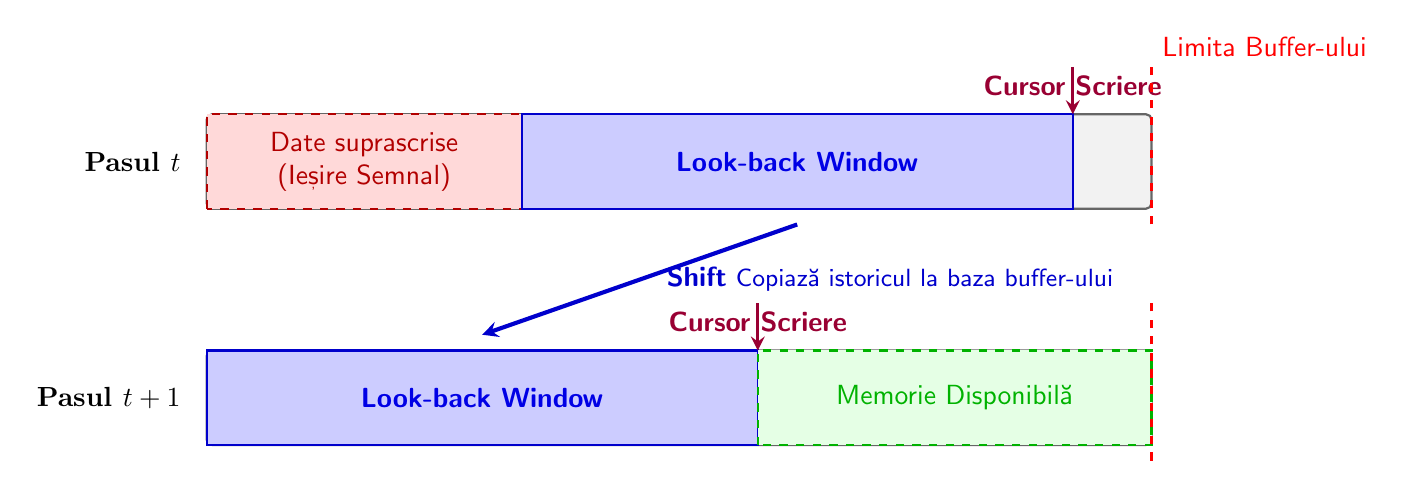
\begin{tikzpicture}[
      font=\sffamily,
      thick,
      >=stealth,
      buffer/.style={draw=black!60, fill=gray!10, minimum width=12cm, minimum height=1.2cm, rounded corners=2pt},
      history/.style={fill=blue!20, draw=blue!80!black, minimum height=1.2cm},
      flushed/.style={fill=red!15, draw=red!70!black, minimum height=1.2cm, dashed},
      free/.style={fill=green!10, draw=green!70!black, minimum height=1.2cm, dashed}
    ]
      \node[buffer] (buf1) at (0, 0) {};

      \draw[flushed]
        (-6, -0.6) rectangle (-2, 0.6)
        node[midway, text=red!70!black, align=center] {Date suprascrise\\(Ieșire Semnal)};
      \draw[history]
        (-2, -0.6) rectangle (5, 0.6)
        node[midway, text=blue!90!black] {\textbf{Look-back Window}};

      \draw[->, very thick, purple!80!black]
        (5, 1.2) -- (5, 0.6)
        node[above=0.1cm] {\textbf{Cursor Scriere}};
      \draw[dashed, very thick, red]
        (6, -0.8) -- (6, 1.2)
        node[above right, text=red] {Limita Buffer-ului};
      \node at (-6, 0) [left=0.2cm, font=\bfseries] {Pasul $t$};

      \draw[->, line width=1.5pt, blue!80!black]
        (1.5, -0.8) -- (-2.5, -2.2)
        node[midway, right=0.2cm, align=left]
          {\textbf{Shift} \small Copiază istoricul la baza buffer-ului};

      \begin{scope}[yshift=-3cm]
        \node[buffer] (buf2) at (0, 0) {};

        \draw[history]
          (-6, -0.6) rectangle (1, 0.6)
          node[midway, text=blue!90!black] {\textbf{Look-back Window}};
        \draw[free]
          (1, -0.6) rectangle (6, 0.6)
          node[midway, text=green!70!black] {Memorie Disponibilă};

        \draw[->, very thick, purple!80!black]
          (1, 1.2) -- (1, 0.6)
          node[above=0.1cm] {\textbf{Cursor Scriere}};
        \draw[dashed, very thick, red] (6, -0.8) -- (6, 1.2);
        \node at (-6, 0) [left=0.2cm, font=\bfseries] {Pasul $t+1$};
      \end{scope}
    \end{tikzpicture}%
    }
  \end{center}
\end{frame}